\section{Evaluación de rendimiento}
Realizando una comparación entre ambas metodologías podemos observar, en la figura \ref{fig:comparativa}, que la búsqueda tabú prioriza a los recursos motorizados para la cobertura de las zonas con mayor nivel de violencia. Lo que a su vez produce un mayor valor en el nivel de violencia cubierto a nivel global.

Además de los resultados indicados anteriormente, cabe resaltar que el algoritmo aquí propuesto soluciona un problema multi-objetivo ya que además de priorizar la cobertura de las zonas con mayores niveles de violencia, intenta cubrir todas las aristas del grafo. Esto último, se puede apreciar fácilmente comparando las figuras \ref{fig:estocastico} y \ref{fig:tabusearch}.
\begin{figure}
    \centering
    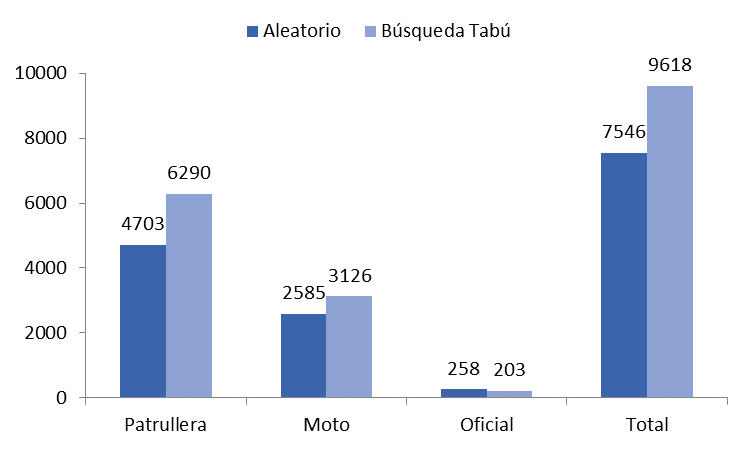
\includegraphics[width=88mm,scale=0.5]{images/comparativa.png}
    \caption{Niveles de violencia cubiertos por tipo de recurso en ambas metodologías.}
    \label{fig:comparativa}
\end{figure}